
\chapter{背景知識}

\section{深層類神經網路}

\subsection{簡介}

  深層類神經網路(Deep Neural Network,DNN)是由神經科學家麥氏(McCulloch)與皮氏(Pitts)於 1943 年提出 \cite{mcculloch_logical_1943} 的計算模型,靈感取自連結主義(Connectionism)的核心主張 --- 以模仿生物神經網路的連結方式模擬複雜的心智活動。

        為模擬神經細胞處理訊號的過程,深層類神經網路最基本的單位稱為「神經元(Neuron)」,其本質為線性分類器。每個神經元接收的輸入數值 $x = (x_1, x_2, \cdots\cdots, x_N)$ 是一個 $N$ 維向量,每一維會被賦予一個權重(Weight) $w = (w_1, w_2, \cdots\cdots, w_N)$  ,加權後總和再加上偏差值(Bias) $b$,得到線性輸出值。為了模擬神經細胞的觸發過程,該分類器常被加上非線性的激發函數(Activation Function)$\sigma$ 的轉換,才得到最終輸出值 $y$。如圖 \ref{fig:single-neuron}所示,神經元的運算規則以下列數學式描述:
\begin{align}
    y = \sigma(w^T x + b)
\end{align}
常見的激發函數包含線性整流單元(Rectified Linear Unit,ReLU)、S 函數(Sigmoid Function)或雙曲正切函數(Hyperbolic Tangent Function,$\tanh$)等等。

\begin{figure}
    \centering
    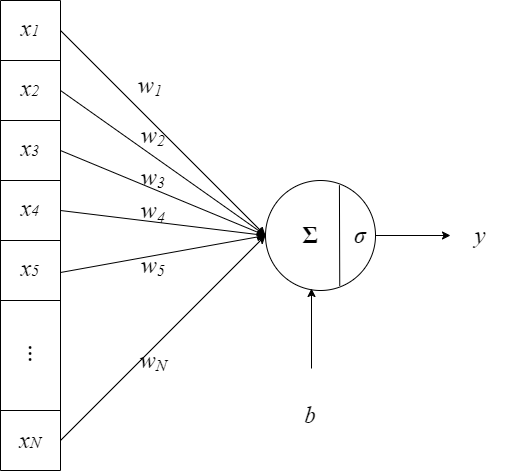
\includegraphics[width=0.5\linewidth]{figures/neuron.drawio.png}
    \caption{神經元示意圖}
    \label{fig:single-neuron}
\end{figure}

        結合數個神經元的運算,羅氏(Rosenblatt)\cite{rosenblatt_perceptron_1958} 於 1958 年提出感知器(Perceptron)模型。根據通用近似定理(Universal Approximation Theorem)\cite{funahashi_approximate_1989} ,感知器理論上可逼近任意函數。然而,後續研究發現單層的感知器具有如「線性不可分」\footnote{例如無法貼合異或(Exclusive OR,XOR)運算等函數} 等先天限制,使其曾經一度不被看好。

        為了突破該缺陷,人們嘗試在輸入與輸出層之間增加「隱藏層(Hidden Layer)」,成為「多層感知器(Multilayer Perceptron,MLP)」,如圖 \ref{fig:mlp} 所示。藉助隱藏層的幫助,多層感知器可對輸入進行多次非線性轉換,大大拓展了模型的適用範圍。此模型是透過「加深隱藏層」得來,現今為人們熟知的「深層類神經網路」即由此得名。

\begin{figure}
    \centering
    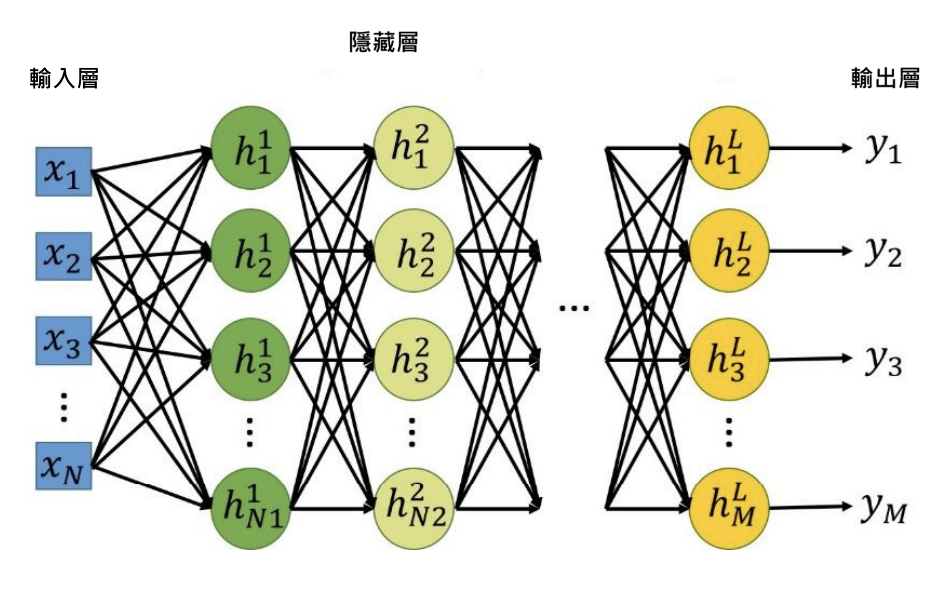
\includegraphics[width=0.8\linewidth]{figures/nnout.png}
    \caption{多層感知器/深層類神經網路示意圖}
    \label{fig:mlp}
\end{figure}
        % 確認那個「大量」跟「應用」有沒有掉字
        藉助深層類神經網路的彈性,我們可以透過大量訓練資料來訓練模型,藉此逼近應用任務中欲近似的函數 $f$,該函數蘊藏在資料集 $\mathcal{D} = \{(x_i, y_i)\}_{i=1}^N$ 中,其中每個資料點 $(x_i, y_i)$ 為輸入與輸出間的配對,即對於 $N$ 個資料點都有 
\begin{align}
    y_i = f(x_i) \ \  \forall i \in \{1, \cdots\cdots, N\}
\end{align}
之關係。為了使這個函數更加逼近目標函數 $f$,類神經網路會構建一個逼近中的函數 $f_{\theta_t}(\cdot)$ 。透過不停的迭代,模型對資料集 $\mathcal{D}$ 的每一筆資料 $x$ 給出預測 $f_{\theta_t}(x)$ 。透過某個減損函數(Loss Function)$\mathcal{L}$ 計算出誤差(Error),此誤差對參數 $\theta_t$ 求出梯度(Gradient)後將指示模型更新的方向,以此乘上學習率(Learning Rate)$\eta$ 後從參數  $\theta_t$ 減去,便能對整個模型進行更新,使之更有機會接近目標函數 $f$。由於此過程是依照梯度使得函數 $\mathcal{L}$ 逐步降低,以此獲名「梯度下降法(Gradient Descent)」,其公式如下:
\begin{align}
    \theta_{t+1} \leftarrow \theta_{t} - \eta \nabla_\theta\mathcal{L}(\mathcal{D}, f_{\theta_t}(\cdot))
\end{align}
其中,$t$ 為當前的迭代數,$\theta_t$ 為當前模型參數,$\theta_{t+1}$ 為更新後的模型參數。

        在此模型更新的過程中,減損函數承擔著指引模型逼近的角色,因此根據應用的任務不同,常見的減損函數包括
\begin{itemize}
    \item 均方誤差(Mean Squared Error,MSE):一般用於迴歸(Regression)問題,直接計算兩數值之間的差距的平方和
          \begin{align}
              \mathcal{L}_{\text{MSE}}(y_i, \hat{y}_i) = \frac{1}{N} \sum_{i=1}^{N} (y_i - \hat{y}_i)^2
              \label{eq:mse}
          \end{align}
          % \textcolor{red}{\(\hat{y}_i\) 是……??????????}

          式 \eqref{eq:mse} 中的 \(\hat{y}_i\) 是模型預測的輸出值,理想上希望愈接近資料標註 \(y_i\) 愈好。
    \item 交叉熵(Cross-entropy,CE):一般用於分類(Classification)問題,著重計算兩個機率分佈之間的差異
          \begin{align}
              \mathcal{L}_{\text{CE}}(y_i, \hat{y}_i) = - \sum_{i=1}^{N} \left[ y_i \log(\hat{y}_i) + (1 - y_i) \log(1 - \hat{y}_i) \right]
          \end{align}
          式中的 \(\hat{y}_i\) 與 \(y_i\) 所代表的意義和式 \eqref{eq:mse} 相同,分別表示模型預測值與資料標註,只是計算兩者差距的方式有異。
\end{itemize}

        透過上述的訓練方式可以得知,類神經網路的訓練需要相當龐大且複雜的運算過程,因此剛提出時仍舊難以應用於現實應用中。

        為了提高函數貼合的效率,魯氏(Rumelhart) \cite{rumelhart_learning_1986} 與辛氏(Hinton) \cite{rumelhart_learning_1987} 等人提出了反向傳播(Back-Propagation)演算法,旨在將上述的更新過程,藉助鏈鎖率(Chain Rule)的幫助,由隱藏層逐層反向傳播至輸入層,對整個類神經網路進行修正。

        反向傳播演算法的設計,正好能配合圖形處理器(Graphics Processing Unit,GPU)等硬體裝置的優勢,以平行運算能力加速函數貼合(Fit)的效率。由此開始,這種透過深層類神經網路,從大量資料集中發掘函數關係的機器學習演算法,被稱為「深層學習(Deep Learning)」。 類神經網路在各個領域的泛化能力(Generalizability)已經得到前所未有的效能,包含電腦視覺、語音處理和自然語言處理,因此深層學習在近年成為人工智慧發展的主流。

        然而,根據資料特性的不同,並不是所有的資料都適用簡單的「輸入與輸出配對」的模式。研究者根據任務需求,發展出了不同架構的類神經網路以適應資料特性。前述最基本的深層類神經網路,由於資料是直接由輸入層,通過逐層的矩陣運算得到輸出,因此被稱之為「前饋式類神經網路(Feed-Forward Network,FFN)」。

        藉由調整各神經元之間的連接關係,發展出卷積式(Convolutional)、遞迴式(Recurrent)與轉換器(Transformer)類神經網路等架構變體,以適應如影像、語音和文字等不同型態的資料。這些架構在語音與文字處理被普遍使用,接下來將逐一分別介紹:

\subsection{卷積式類神經網路}

  卷積式類神經網路(Convolutional Neural Network,CNN)為 1998 年由楊氏(LeCun) \cite{lecun_gradient-based_1998} 提出,旨在以訊號處理的卷積(Convolution)運算,模擬生物的視覺皮質感知 \cite{hubel_receptive_1959} 。

\begin{figure}
    \centering
    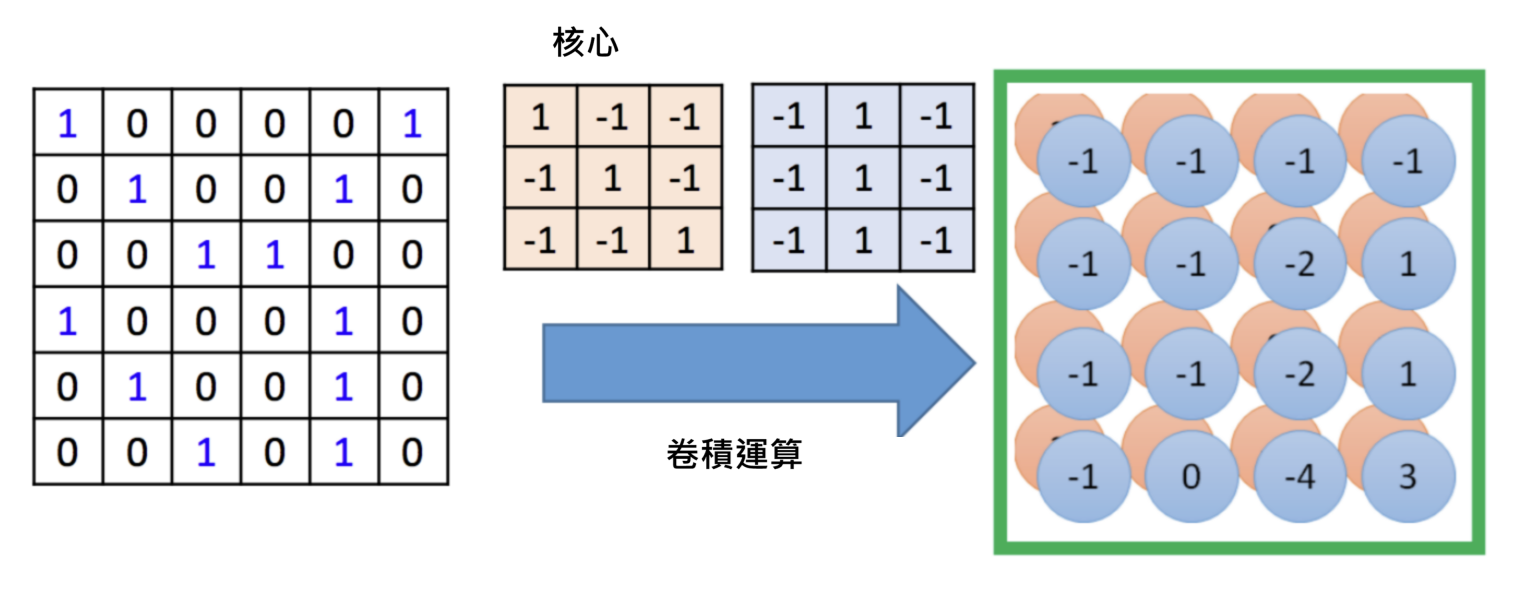
\includegraphics[width=0.9\linewidth]{figures/cnnnew.png}
    \caption{卷積式類神經網路示意圖,取自李宏毅教授的課程投影片}
    \label{fig:cnn}
\end{figure}

        如圖 \ref{fig:cnn} 所示,卷積式類神經網路透過核心(Kernel),對輸入的資料 --- 如圖中的二維矩陣 --- 進行卷積運算,獲得該輸入的特徵圖(Feature Map)。核心帶來的移動不變性(Shift-invariance)非常適用於捕捉二維影像中的局部特徵,以作為類神經網路分辨資料的依據。

        有別於影像處理中,資料多以二維矩陣表示像素 (Pixel)三原色的亮度數值,因此以二維的卷積運算為主;由於語音時常處理時間軸之上的訊號,包含聲波波形(Waveform)、時頻譜(Spectrogram)或聲學特徵,因此一維的卷積式模型也時常出現,以模仿人耳聽覺對時變訊號的窗框(Window)的效應,進而觀察到語音中在不同解析度(Resolution)的資訊。

\subsection{遞迴式類神經網路與序列至序列模型}

\subsubsection{遞迴式類神經網路}

  遞迴式類神經網路(Recurrent Neural Network,RNN)常用於處理隨時間變化的序列資料,特別是語音與文字等等,順序資訊相當關鍵的各種語言任務。為了處理需要記憶和狀態的資料類型,遞迴式類神經網路的輸出會重新接回輸入層,使得前一個時間點(Timestep)的資料與內部狀態會繼續影響後續的時間點。常用的遞迴式類神經網路類型有長短期記憶(Long Short-term Memory,LSTM)\cite{hochreiter1997long} 和閘門循環單元(Gated Recurrent Unit,GRU)\cite{cho-etal-2014-properties} 等。

        遞迴式類神經網路通常用在處理序列至序列的應用,例如語音辨識、語音合成或機器翻譯等和語言密切相關的任務中。

\subsubsection{序列至序列模型}

  由於許多語言資料通常以兩個序列互相配對的形式呈現,因此專門處理這類資料的模型被稱為「序列至序列模型(Sequence-to-sequence,Seq2seq)」\cite{sutskever2014sequence}。此類模型的典型架構由編碼器(Encoder)和解碼器(Decoder)組成,旨在模擬輸入與輸出序列之間的變化與相依關係(Dependency)。

        序列到序列模型一般有兩種模式:其一是每個時間點都生成一個輸出的向量,適用於輸入與輸出序列等長的任務,這種模式被稱為「符記分類(Token Classification)」;但更常見的情況是,輸入與輸出序列的長度並不相同。處理後者的典型作法是讓編碼器將輸入序列依據時間,一步一步輸入編碼器,將序列編碼為內部表徵(Latent Representation)。完成編碼後,編碼器將最後一個時間點的表徵用以代表整個序列,稱為「語境向量(Context Vector)」。該向量接著被傳遞給解碼器,依序生成輸出序列。

\subsection{專注機制與轉換器類神經網路}

\subsubsection{專注機制(Attention Mechanism)}

  由於遞迴式類神經網路需要處理整個序列的編碼和解碼資訊,對時間點距離較遠的輸入容易被遺忘,亦即難以處理長期相依性(Long-term Dependency)問題。為了解決這種困境,巴氏(Bahdanau)等人\cite{bahdanau2014neural} 提出了「專注機制」。該機制讓解碼器將輸入序列的每個訊號都視作「部分的」語境向量,由對不同時間點的向量加權合計獲得,使得在生成輸出序列時能依據當時的需求從輸入序列中提取所需的訊息。專注機制的引入,使得序列至序列模型在處理如語音辨識、機器翻譯等任務時效能大大改善。

\subsubsection{轉換器類神經網路}

  儘管遞迴式類神經網路善於處理時序資料,但其難以平行化的架構限制了其在訓練和推理(Inference)時的效率。2017 年,瓦氏(Vaswani)等人 \cite{vaswani2017attention} 提出了完全由專注機制構成、不依賴遞迴運算的序列至序列模型,並稱之為「轉換器(Transformer)」,以解決機器翻譯等任務。

        轉換器類神經網路一般包含編碼器和解碼器兩部分,均為多層架構。圖 \ref{fig:tfm_arch} 展示完整的轉換器架構圖,以下分別介紹其主要元件:

\paragraph{位置編碼(Positional Encoding)} \hfill \break
%
  對於編碼器或解碼器的輸入序列,模型先對序列中不同位置的時間點進行編碼,取代遞迴式類神經網路逐步運算的過程,使其能在平行計算的同時考慮不同時間點的影響。編碼的函數可依照需求變換,如原始的轉換器採用三角函數進行位置編碼,而在語音模型中,有時也會採用卷積式網路以捕捉輸入的細微資訊。

        經過位置編碼後,向量會通過每一個轉換器層(Transformer Layer),進行以「多頭專注」為主的一連串運算:

\paragraph{多頭專注(Multi-head Attention)} \hfill \break
%
  轉換器層中的專注機制涉及三個輸入向量:詢向量(Query)$Q$、鑰向量(Key)$K$ 和值向量(Value)$V$。專注機制運算如下:
\begin{align}
    \text{Attention}(Q, K, V) = \text{softmax}
    \left(
    \frac{QK^\top}{\sqrt{d_k}}
    \right)
    V
                \label{eq:attn}
\end{align}
其中 $\text{softmax}$ 為正規化指數函數,$d_k$ 為鑰向量 $K$ 的維度。這一運算首先通過鑰向量和詢向量的內積計算專注權重,而後為避免受維度過大影響而縮小為 $\sqrt{d_k}$ 分之一,最後通過正規化指數函數使得權重總和為 1 ,以此分配給值向量進行加權。

        為應對多樣的輸入訊號,每個轉換器層具備多個獨立的專注機制,對三組輸入向量先進行各自不同的 $W^Q$、$W^K$、$W^V$ 線性轉換,稱為「多頭專注」。對於第 $i$ 個專注頭(Head)有
\begin{align}
    \text{head}_i = \text{Attention}(QW^Q_i,KW^K_i,VW^V_i)
\end{align}
          % \textcolor{red}{\(\text{Attention}(\cdot, \cdot, \cdot)\) 是……??????????} \\
也就是每個專注頭分別透過前述式 \eqref{eq:attn} 的 \(\text{Attention}(\cdot, \cdot, \cdot)\) 運算,使模型針對不同輸入訊號可以入進行不一樣的運算處理。最後,若有 $h$ 個專注頭,多頭專注模組會將多個頭的結果進行串接(Concatenate,即式 \eqref{eq:multihead} 描述之 \( \text{Concat} \)),經過線性轉換 $W^O$ 作為模組輸出,運算式表示為
\begin{align}
    \text{MultiHead}(Q, K, V) = \text{Concat}(\text{head}_1, \cdots\cdots, \text{head}_h) W^O
    \label{eq:multihead}
\end{align}
最終將 \(\text{MultiHead}(Q, K, V)\) 作為整個多頭專注模組的輸出值。

\paragraph{其他層內運算} \hfill \break
%
  每層轉換器層在經過多頭專注運算後,會依序進行以下三個步驟:

\begin{enumerate}
    \item 與輸入向量透過殘差連接(Residual Connection)相加,隨後進行層正規化(Layer Normalization)以穩定訓練。
    \item 將此結果通過一個簡單的前饋式類神經網路對向量做線性轉換。
    \item 再將前饋網路的輸入與輸出再次計算殘差總和後,進行層正規化輸出。
\end{enumerate}

        以上為轉換器被提出時的最原始模型,其後對殘差連接、層正規化的安排也存在各類變體。

\paragraph{跨專注機制(Cross-atttention)} \hfill \break
%
  解碼器為了輸出資訊,需要來自編碼器的輸入序列,因此原本在編碼器層中的自專注機制,在解碼器中會再經過一次跨專注機制的運算,使用編碼器提供的詢向量和鑰向量對解碼器的值向量進行專注運算。
\begin{figure}
    \centering
    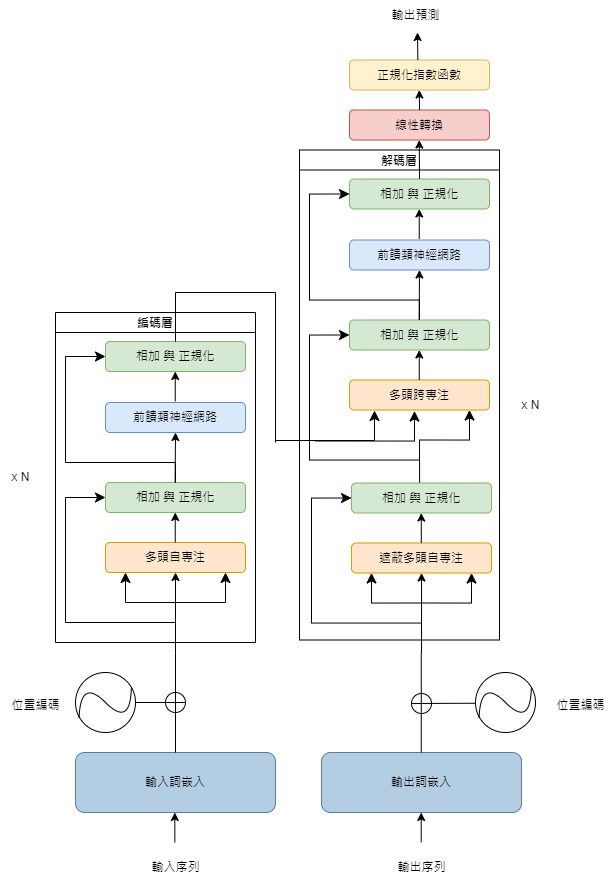
\includegraphics[width=0.9\linewidth]{figures/tfm_arch.drawio.png}
    \caption{轉換器架構圖}
    \label{fig:tfm_arch}
\end{figure}
        由於轉換器不需要對每個時間點逐一運算,使此過程能被高度平行化,類神經網路得以透過專注機制同時進行序列資料的大量訓練。這種可擴展性(Scalability)使其在自然語言和語音處理上取得了巨大的進展,幾乎取代了原先遞迴式類神經網路的應用場景,近年來甚至被應用在圖像類的資料上\cite{dosovitskiy2021image},展現了此種模型架構的彈性與泛用性,成為目前最前沿的人工智慧主流架構。

        除了模型架構,機器學習中不可或缺的另一大部分是對資料的編碼過程。如何更有效率的讓機器理解、處理和輸出資料,是機器學習乃至深層學習的一大課題。面對捉摸不定、抽象且變化萬千的人類語言,語音和文字處理中的表徵學習尤為重要。

\section{表徵與自監督式學習}

\subsection{特徵抽取與表徵學習}

  不論採用何種模型,為了讓機器可以處理並捕捉輸入資料中的訊號與規律,包括如何對資料編碼和運算的步驟,在機器學習中稱之為特徵抽取(Feature Extraction)或表徵學習(Representation Learning),這是模型建構中不可或缺的重要步驟。

        對於抽象的語言概念,早期工程領域根據對語音和文字的理解,分別進行了不同的處理。對於離散且可計數的文字,人們使用詞頻統計衍生出如 \(n\) 連詞(\(n\)-gram)、TF-IDF(詞頻-倒數文件頻率,Term-Frequency Inverse Document Frequency)等特徵作為模型學習的前處理步驟;而對於連續且複雜的語音,工程師則透過聲學原理與訊號處理的知識,使用如濾波器組(Filter Bank)、梅爾倒頻譜係數(Mel-Frequency Cepstrum Coefficient,MFCC)等特徵,類比人耳捕捉語音訊號的過程。

        在深層學習逐漸發展的過程中,自然語言處理領域的一大里程碑是米氏(Mikolov)提出的「Word2vec」模型 \cite{mikolov_efficient_2013},該模型以連續的向量表徵(Vector Representation)取代稀疏(Sparse)的統計數據,對離散的文字單詞進行「詞嵌入(Word Embedding)」編碼。通過大量文本運算,將各單詞之間的共現(Collocation)以跳躍詞(Skip-gram,SG)、連續詞袋(Continuous Bag-of-Word,CBOW)等演算法轉換成高維向量空間中的點,找出每個單詞最適合的語義表徵。爾後,為了更細緻地捕捉同一單詞在不同句子中的脈絡變化,ELMo(來自語言模型的詞嵌入,Embeddings From Language Model)\cite{peters_deep_2018} 提出了「含上下文詞嵌入(Contextualized Embedding)」的概念,使得各單詞在運算表徵的過程中可以根據上下文進行些微調整。

\subsection{自監督學習}

  隨著轉換器模型的提出,BERT(來自轉換器的雙向編碼器表徵,Bidirectional Encoder Representations From Transformers)\cite{devlin_bert_2019} 被提出。通過自專注機制,工程師們無需依賴人工標記,透過預先設定任務(Pretext Task)引導模型從大量文本中自行找出更細緻且考量前後文的語義關係,並在許多文字任務上獲得了優異的成績。

        自此,楊氏(LeCun)將這種以特定任務作為引導、藉助資料本身的結構替代標註,從大量未標註資料中學習資料規律的訓練方式,稱之為「自監督學習(Self-supervised Learning,SSL)」。BERT 的成功使自監督學習得以大行其道,並出現了許多由巨量資料進行預訓練(Pre-train)的基石模型(Foundation Model),有效解決了語言處理領域中的標註資料稀缺的問題。人們在解決語言相關任務時,不需從頭蒐集資料與進行耗時耗能的訓練過程,而是可以利用基石模型優良的泛化(Generalization)能力,解決各種應用任務的需求。相比於預訓練的任務,這些更貼近日常現實的任務被稱為「下游任務(Downstream Task)」,能應對廣泛的下游任務種類,這是基石模型最大的優勢。

        有鑑於文字處理方面的成功,語音領域的研究者嘗試將相似模式應用於語音,眾多語音基石模型隨之出現。大量的語音資料庫幫助模型萃取出有助於下游任務的語音表徵(Speech Representation),在各種任務上獲得了優於傳統聲學特徵的表現。語音表徵具備的無窮潛力,逐漸成為聲學特徵之外的新選擇。

        依照這些語音自監督模型的預訓練學習模式,可大致分為重建式、預測式與對比式模型。以下分別介紹這三類模式:

\subsubsection{重建式學習(Reconstruction Learning)}

  此類模型通過對輸入訊號進行擾動(Perturb)後,期望模型將被更動的輸入重新預測回原始資料,通常減損函數表示為:
\begin{align}
    \mathcal{L}_{recon} = \mathbb{E}_x[|f_\theta(\tilde{x}) - x|]
\end{align}
其中 $\tilde{x}$ 為擾動後的資料,$f_\theta(\cdot)$ 為模型函數。擾動方式通常以遮蔽為主,在文字處理中以 BERT 為代表,稱為「遮蔽語言模型(Masked Language Model,MLM)」。在語音中,採用此方式學習的有 Mockingjay \cite{liu_mockingjay_2019}、TERA \cite{t_tera_2021} 等模型。  % NPC

\subsubsection{預測式學習(Predictive Learning)}

  此類模型通過預訂一些學習目標函數,製造類似輸入與輸出的配對資料,讓模型預測該函數的結果來學習資料中的特定結構。其訓練減損函數可表示為:
\begin{align}
    \mathcal{L}_{pred} = \mathbb{E}_x[\text{eval}(f_\theta(x), \hat{f}(x))]
\end{align}
其中 $\hat{f}$ 是期望模型學習的目標函數,$f_\theta(\cdot)$ 為模型函數,$\text{eval}$ 是用來評估預測好壞的標準。

        目標函數的典型代表是自迴歸(Autoregressive),期望模型預測未來時間點的輸入表徵。文字方面以「GPT(生成式預訓練轉換器,Generative Pretrained Transformer)」系列 \cite{radford_language_nodate, brown_language_2020} 為代表,語音上的「自迴歸預測編碼(Autoregressive Predictive Coding,APC)」 \cite{chung_generative_2020} 也是採用此種模式。此外,語音基石模型還可以使用其他訓練目標,如 PASE+ \cite{ravanelli_multi-task_2020} 預測其他模型的表徵,而本文著重探究的「HuBERT(隱藏單元 BERT,Hidden-unit BERT)」\cite{hsu_hubert_2021, hsu_hubert_2021-2} 則以預測分群(Cluster)後的輸入表徵為目標,這些預測目標又被視為虛擬標註(Pseudo-label),後文將著重探討。

\subsubsection{對比式學習(Contrastive Learning)}

  此學習方式的訓練目標是要求模型區分正樣本(Positive Sample)與負樣本(Negative Sample)的差異,減損函數通常定義為:
\begin{align}
    \mathcal{L}_{contr} = -\mathbb{E}_x\left[\log
        \left(
        {\frac
            {\sum_{\tilde{x} \in x_{pos}}\exp(\text{sim}(x, \tilde{x}))}
            {\sum_{\tilde{x} \in \mathcal{X}}\exp(\text{sim}(x, \tilde{x}))}
        }\right)\right]
\end{align}

        其中 $x$ 為輸入,$x_{pos}$ 為正樣本,$\mathcal{X}$ 為包含正負樣本的資料集,$\text{sim}(\cdot, \cdot)$ 是評估兩個樣本相似程度的函數,常用的相似度函數為內積運算得出的餘弦相似度(Cosine Similarity)。語音上最早使用對比式學習的模型為「對比預測編碼(Contrastive Predictive Coding,CPC)」\cite{maekaku2022speech},之後如 Wav2vec \cite{schneider2019wav2vec}、Modified CPC \cite{rivière2020unsupervised}、Wav2vec 2.0 \cite{baevski2020wav2vec} 等模型亦是以對比正負樣本的模式訓練,但訓練時正負樣本的定義有所差異,如 Wav2vec 僅以時間維度上相同的向量為正樣本,其餘則將固定時間內的向量皆視為正樣本。

        對比式學習通過正負樣本的定義,將預訓練任務形塑為分類問題,因此減損函數本質上為交叉熵,使模型能夠判斷訓練資料中的結構差異。

\subsection{向量量化與離散單元}

  語音訊號雖然記錄語言資訊,卻與影像資料一樣都是連續數值資料,不像離散的文字較易處理,因此發展出了許多應用廣泛的模型。為了使語音模型訓練可以套用自然語言處理領域的演算法,從連續語音中找出離散表徵逐漸成為研究趨勢,這類研究被稱為「聲學單元發掘(Acoustic Unit Discovery,AUD)」。

        由於語言概念本質上是離散符號,向量量化技術常用於涉及語言標註的情境,如電腦視覺經典的量化向量變分自編碼器(Vector-Quantized Variational Autoencoder,VQ-VAE)\cite{van2017neural},利用影像標註的離散語言單詞特性,使模型學習的表徵向量被約束在編碼簿(Codebook) 的幾個向量中。

        在語音領域,基於 Wav2vec 之上的 Vq-wav2vec \cite{baevski2019vq} 和 Wav2vec 2.0 將連續的語音特徵量化加入訓練目標中,在語音辨識等任務上取得了顯著進步。

        HuBERT \cite{hsu_hubert_2021-2} 則先對連續的 MFCC 特徵進行 K-平均(K-Means)演算法分群,以所得的群心(Centroid)或碼字(Code Word)編號作為訓練目標,實施類似 BERT 的遮蔽語言模型訓練,並改以此次訓練得到的語音表徵為目標,再次分群後實施第二次訓練。這些經過兩輪訓練後,從模型表徵分群得到的群心,被視為「隱藏單元(Hidden Unit)」,呈現了語音訊號中的代表性聲學特徵。透過找出隱藏單元的過程,HuBERT 在低資源情況下達到與 Wav2vec 2.0 相近的語音辨識成績。

\subsection{無文字(Textless)架構}

  奠基於 HuBERT 等語音基石模型的成功,利用隱藏單元的概念,將大量語音資料表徵進行 K-平均演算法,作為這些語音訊號的虛擬標註。如此得到的大量離散隱藏單元形成了「虛擬文字(Pseudo-text)」的語料庫,基於這些離散單元訓練的語言模型,稱為「生成式口語語言模型(Generative Spoken Language Model,GSLM)」\cite{lakhotia_generative_2021-1}。配合反向語音合成訓練基於離散單元的語音生成模型,整體架構完全不依賴文字標註,訓練出純語音語言模型,稱為「無文字(Textless)架構」\cite{noauthor_textless_2021}。

        無文字模式在語音問答(Spoken Question Answering)\cite{lin2022dual}和語音到語音翻譯 (Speech-to-speech Translation)\cite{chen_speech--speech_2023}中取得了前所未有的進展。這些「離散單元(Discrete Unit)」被視為類似文字卻不依賴人類文字標記的語音表徵,具有儲存位元率低和可套用文字語言模型訓練模式的優勢,受到語音社群的廣泛借鑑,後續也帶出了許多如\cite{zhang2024speechtokenizer} 等將語音以離散表徵編碼的研究。

        雖然在系統與應用任務上取得了成功,但這些離散單元本身與文字的差異,及其對語音語言模型訓練的幫助,仍是領域內探討的焦點。有鑑於此,本論文基於語言知識,從最接近文字且與語音訊號最相關的「音位(Phoneme)」開始探討,期望了解離散單元能帶來的特徵及其對後續應用的幫助。

\section{本章節總結}

  本章節首先介紹了深層學習模型的核心部件 --- 類神經網路的基本原理,隨後對本論文研究的核心 --- 「語音表徵」與「離散單元」的發展與歷史進行了梳理。接下來的章節將緊扣這些基石模型得到的離散特徵,對其與「音位」這類語音學標記之間的統計關係進行更深入分析。
